%COMANDO CHE DETERMINA IL TIPO DI DOCUMENTO CHE SI VUOLE CREARE

\documentclass[a4paper,12pt]{report}

%ELENCO DEI PACCHETTI UTILI PER LA STESURA DEL DOCUMENTO
\usepackage{enumitem}
\usepackage[utf8]{inputenc}
\usepackage[english, italian]{babel}
\usepackage{graphicx}
\usepackage{float}
\usepackage{tabularx}
\usepackage{makecell}
\usepackage{titlesec}
\usepackage{fancyhdr}
\usepackage{lastpage}
\usepackage{xurl}
\usepackage{hyperref}
\usepackage{geometry}
\usepackage[table,dvipsnames]{xcolor}
\setcounter{tocdepth}{5}
\setcounter{secnumdepth}{5}
\usepackage{caption}
\usepackage{etoolbox}% >= v2.1 2011-01-03
\usepackage{tikz}
\usepackage{listings}
\usepackage{scalerel}
\usepackage{longtable}
\captionsetup[table]{position=bottom}
\usepackage{comment}
\titleformat{\chapter}[display]
{\normalfont\bfseries}{}{0pt}{\LARGE}

%COMANDO PER LA SPAZIATURA DEI TITOLI DAL BORDO DEL FOGLIO

\titlespacing*{\chapter}{0cm}{0cm}{0.2cm}

%COMANDO PER LA SPAZIATURA DEL TESTO DAI BORDI LATERALI

\geometry{
	left=20mm,
	right=20mm,
}

%COMADNO PER AVERE L'INDICE DEL NOME CHE SI VUOLE

\renewcommand{\contentsname}{Indice}

%COMADNI PER OTTENERE SUBSUBSECTION NUMERATE E PRESENTI NELL'INDICE

\setcounter{tocdepth}{5}
\setcounter{secnumdepth}{5}

%COMANDI PER OTTENERE HEADER E FOOTER

\pagestyle{plain}

\fancypagestyle{plain}{
	\fancyhf{}
	\lhead{
\includegraphics[width=3cm]{../../immagini/minilogo.jpg}}
	\chead{}
	\rhead{\fontsize{12}{10}Verbale Esterno 2021-04-15}
	\lfoot{}
	\cfoot{\thepage\ di \pageref{LastPage}}
	\rfoot{}
}

\pagestyle{plain}

%COMANDI PER LINK

\hypersetup{
	colorlinks=true,
	linkcolor=black,
	filecolor=black,
	urlcolor=blue,
	citecolor=black,
}

%COMANDI PER SNIPPET DI CODICE

\BeforeBeginEnvironment{lstlisting}{\begin{mdframed}\vspace{-0.7em}}
	\AfterEndEnvironment{lstlisting}{\vspace{-0.5em}\end{mdframed}}

% needed for \lstcapt
\def\ifempty#1{\def\temparg{#1}\ifx\temparg\empty}

% make new caption command for listings
\usepackage{caption}
\newcommand{\lstcapt}[2][]{%
	\ifempty{#1}%
	\captionof{lstlisting}{#2}%
	\else%
	\captionof{lstlisting}[#1]{#2}%
	\fi%
	\vspace{0.75\baselineskip}%
}

\definecolor{atomlightorange}{rgb}{0.88,0.76,0.55}
\definecolor{atomdarkgrey}{RGB}{59,62,75}

% set listings
\lstset{%
	basicstyle=\footnotesize\ttfamily\color{atomlightorange},
	framesep=20pt,
	belowskip=10pt,
	aboveskip=10pt
}

% add frame environment
\usepackage[%
framemethod=tikz,
skipbelow=8pt,
skipabove=13pt
]{mdframed}
\mdfsetup{%
	leftmargin=0pt,
	rightmargin=0pt,
	backgroundcolor=atomdarkgrey,
	middlelinecolor=atomdarkgrey,
	roundcorner=6
}

%BIBLIOGRAFIA

\makeatletter
\def\thebibliography#1{\chapter*{Bibliografia\@mkboth
		{Bibliografia}{Bibliografia}}\list
	{[\arabic{enumi}]}{\settowidth\labelwidth{[#1]}\leftmargin\labelwidth
		\advance\leftmargin\labelsep
		\usecounter{enumi}}
	\def\newblock{\hskip .11em plus .33em minus .07em}
	\sloppy\clubpenalty4000\widowpenalty4000
	\sfcode`\.=1000\relax}
\makeatother

%DEFINIZIONE COLORI

\definecolor{airforceblue}{rgb}{0.36, 0.54, 0.66}

\begin{document}

\makeatletter
\begin{titlepage}
	\begin{center}
		\vspace*{-4,0cm}
		\author{Jawa Druids}
		\title{Analisi dei Requisiti}
		\date{} %LASCIARE QUESTO CAMPO VUOTO, SE LO TOLGO STAMPA LA DATA CORRENTE
		
\includegraphics[width=0.5\linewidth]{../immagini/DRUIDSLOGO.jpg}\\[4ex]
		{\huge \bfseries  \@title }\\[2ex]
		{\LARGE  \@author}\\[50ex]
		\vspace*{-9,0cm}
		\begin{table}[H]
			\renewcommand{\arraystretch}{1.4}
			\centering
			\begin{tabular}{r | l}
				\textbf{Versione} & v3.0.0 \\%RIGA PER INSERIRE LA VERSIONE ULTIMA DEL DOCUMENTO
				\textbf{Data approvazione} & 15-03-2021\\
				\textbf{Responsabile} & Mattia Cocco\\
				\textbf{Redattori} & \makecell[tl]{ Margherita Mitillo } \\
				\textbf{Verificatori} & \makecell[tl]{Andrea Dorigo \\ Mattia Cocco \\Alfredo Graziano } \\
				%MAKECELL SERVE PER POI ANDARE A CAPO ALL'INTERNO DELLA CELLA
				\textbf{Stato} & Approvato\\
				\textbf{Lista distribuzione} & \makecell[tl]{Jawa Druids \\ Prof. Tullio Vardanega \\ Prof. Riccardo Cardin \\ Sync Lab}\\
				\textbf{Uso} & Esterno
			\end{tabular}
		\end{table}
		\vspace{0.2cm}
		\hfill \break
		\fontsize{17}{10}\textbf{Sommario} \\
		\vspace{0.3cm}
		L'\emph{\normalsize Analisi dei Requisiti} individua tutti i requisiti da implementare nel prodotto da sviluppare.
	\end{center}
\end{titlepage}
\makeatother

\def\myformat#1{
	\centering\huge#1
}
\hfill \break
\section*{\myformat{Registro delle modifiche}}
{\rowcolors{2}{Apricot!90!Bittersweet!20}{Bittersweet!70!Apricot!40}

\begin{table}[H]
	\centering
	\begin{tabular}{|c|c|c|c|c|}
		\hline
		\rowcolor{Melon} 
		\textbf{Modifica} & \textbf{Autore} & \textbf{Ruolo} & \textbf{Data} & \textbf{Versione}\\
		\hline
		\textit{Prima stesura bozza} & Andrea Dorigo & \textit{Responsabile} & 26-11-2020 & v0.0.1 \\
		\hline
	\end{tabular}
\end{table}

%COMANDO PER LA CREAZIONE DELL'INDICE

\tableofcontents{}
\listoftables{}
\listoffigures{}
\chapter{Introduzione}

\section{Scopo del documento}
Lo scopo del documento è quello di formalizzare i contenuti e le qualità che il prodotto sviluppato dovrà raggiungere. 
I requisiti sono stati individuati attraverso lo studio del capitolato e incontri con l'azienda proponente \textit{Sync Lab}. 
Il documento inoltre è necessario a:
\begin{itemize}
	\item descrivere accuratamente tutti i requisiti proposti dal proponente;
	\item comprendere da parte del committente quali sono le richieste del cliente;
	\item definire il formato e contenuto di ogni requisito specifico del software.
\end{itemize} 
\section{Scopo del prodotto}
In seguito alla pandemia del virus COVID-19 è nata l'esigenza di limitare il più possibile i contatti fra le persone, specialmente evitando la formazione di assembramenti. Il progetto \textit{GDP: Gathering Detection Platform} di \textit{Sync Lab} ha pertanto l'obiettivo di \textbf{creare una piattaforma in grado di rappresentare graficamente le zone potenzialmente a rischio di assembramento, al fine di prevenirlo.}
\\
Al tal fine il gruppo \textit{Jawa Druids} si prefigge di sviluppare un prototipo software in grado di acquisire, monitorare ed analizzare i molteplici dati provenienti dai diversi sistemi e dispositivi, a scopo di identificare i possibili eventi che concorrono all'insorgere di variazioni di flussi di utenti. Il gruppo prevede inoltre lo sviluppo di un'applicazione web da interporre fra i dati elaborati e l'utente, per favorirne la consultazione.
\section{Glossario}
All'interno della documentazione viene fornito un \textit{Glossario}, con l'obiettivo di assistere il lettore specificando il significato e contesto d'utilizzo di alcuni termini strettamente tecnici o ambigui, segnalati con una \textit{G} a pedice.

\section{Riferimenti}
\subsection{Riferimenti normativi}
\begin{itemize}
	\item \textit{Norme di Progetto v1.0.0;}
		\item \textit{Verbale Esterno 17-12-2020;}
		\item \textit{Capitolato d'appalto C3:} \\ \url{https://www.math.unipd.it/~tullio/IS-1/2020/Progetto/C3.pdf}
\end{itemize}
\subsection{Riferimenti informativi}
\begin{itemize}
	\item \textit{Presentazione del capitolato:} \\ \url{https://www.math.unipd.it/~tullio/IS-1/2020/Progetto/C3.pdf}
		\item \textit{Materiale didattico relativo all'Analisi dei Requisiti del corso di Ingegneria del Software:}\\ \url{https://www.math.unipd.it/~tullio/IS-1/2020/Dispense/L07.pdf}
	\item \textit{IEEE Recommended Practice for Software Requirements Specifications:}\\
		\url{https://ieeexplore.ieee.org/document/720574}
	\item \textit{Seminario per approfondimenti tecnici del capitolato C3:}\\
		\url{https://www.math.unipd.it/~tullio/IS-1/2020/Progetto/ST1.pdf}	
		%aggiungere capitolato c3 pdf	
\end{itemize}
\chapter{Descrizione generale}
\section{Caratteristiche del prodotto}
L'idea del capitolato \textit{GDP - Gathering Detection Platform} è di creare una piattaforma che riesca a rappresentare mediante visualizzazione grafica zone potenzialmente a rischio di assembramento e cercare di prevenirle.
La piattaforma utilizzerà dati prelevati da sensori (come telecamere, dispositivi contapersone, etc.) o sorgenti dati (come flussi di prenotazioni Uber, le tabelle degli orari di autobus/metro/treno, etc.), i quali mediante la loro elaborazione verranno rappresentati tramite una \textit{heat-map}.

\section{Funzionalità generali}
Il capitolato \textit{GDP} individua tre principali funzionalità da sviluppare:
\begin{itemize}
	\item Acquisizione di dati: l'acquisizione avverrà attraverso sistemi di monitoraggio e motori software "contapersone" applicati ad immagini/stream delle videocamere;
	\item Elaborazione di dati: i dati verranno elaborati per generare valore aggiunto agli stessi e confrontare flussi diversi di informazioni;
	\item Rappresentazione di dati: attraverso un sito web i dati elaborati verranno visualizzati a video mediante una \textit{heat-map}.
\end{itemize}

\section{Caratteristiche utente}
Il progetto è rivolto principalmente ad utenti di tipo amministrativi, cioè i quali devono visualizzare l'intera mappa di una regione per motivi lavorativi.
%specifica delle conoscenze necessarie per usare l'heat-map/ applicazione

%\chapter{Fasi del progetto}\label{fasiProgetto}
In questo capitolo verranno illustrate le fasi del progetto identificate dal capitolato$_{\scaleto{G}{3pt}}$ d'appalto \textit{GDP-Gathering Detection Platform}. Il capitolo viene diviso nelle tre fasi generali del progetto: acquisizione, elaborazione e visualizzazione dei dati. Secondo lo \textbf{IEEE Standard 830-1998} in questo capitolo verranno spiegati tutti i punti da sviluppare e nel capitolo successivo i requisiti da implementare per la creazione del prodotto richiesto da \textit{Sync Lab}. La descrizione delle fasi è stata inserita in quanto ritenuta necessaria per il chiarimento della necessità dei requisiti individuati. %inserire descrizione requisiti da ISOIEE

\section{FC1: Acquisizione dati}\label{fasiProgettoAquisizioneDati}%FC fase capitolato
In questa sezione vengono descritte le fasi di acquisizione dei dati.

\subsection{FC1.1: Acquisizione con Java}\label{fasiProgettoAquisizioneDatiJava}

\begin{itemize}
	\item \textbf{Descrizione}: attraverso il linguaggio Java$_G$ si creerà un programma che preleva informazioni da sorgenti esterne e le invia al server.
	\item \textbf{Linguaggio di programmazione}: Java$_{\scaleto{G}{3pt}}$.
	\item \textbf{Input}: i dati forniti saranno prelevati da siti con live-feed$_G$ di webcam di varie città e simulatori di spostamenti di persone.
	\item \textbf{Output}: i dati resteranno immutati.
	\item \textbf{Risposta ad errori}: nel caso di mancanza di risposta dai siti con live-feed il programma si bloccherà ed invierà un segnale di errore al server.
\end{itemize}

%sono dubbioso su 1.2 e 1.3 dovrò modificare qualcosa

\subsection{FC1.2: Database}\label{fasiProgettoAquisizioneDatiDatabase}

\begin{itemize}
	\item \textbf{Descrizione}: creazione del database e archiviazione dei dati in esso per visualizzazione future e mantenimento dei dati;
	\item \textbf{Linguaggio}: NoSQL.
\end{itemize}

\subsection{FC1.3: Apache Kafka$_G$}\label{fasiProgettoAquisizioneDatiApacheKafka}

\begin{itemize}
	\item \textbf{Descrizione}: impostazione di una piattaforma di data streaming$_G$ che consente di gestire e trasferire grandi volumi di dati in tempo reale, abbassando notevolmente i tempi di latenza;
	\item \textbf{Input}: flussi di dati dall'acquisizione con Java$_{\scaleto{G}{3pt}}$;
		\item \textbf{Output}: il flusso di dati rimane immutato.
\end{itemize}

%??? I dati verranno inseriti all'interno di un database, questo sarà sviluppato usando Apache Kafka un sistema distribuito che consiste di server e client i quali comunicano tra loro attraverso un protocollo di rete performante di tipo TCP. ???(non so dove inserire)

\section{FC2: Elaborazione Dati}\label{fasiProgettoElaborazioneDati}
Completata la fase precedente i dati verranno elaborati attraverso librerie di Scikit-learn e TensorFlow con il linguaggio di programmazione Python$_G$.
Di seguito vengono individuate le fasi da seguire per l'elaborazione dei dati.

\subsection{FC2.1: Esplorazione Dati}\label{fasiProgettoElaborazioneDatiEsplorazioneDati}

\begin{itemize}
	\item \textbf{Descrizione}: si discriminano elementi all'interno del dataset che portano a predizioni errate del modello.
	\item \textbf{Input}: i dati vengono prelevati dal database.
	\item \textbf{Output}: i dati controllati vengono aggiunti in appositi spazi per individuare la loro correttezza.
	\item \textbf{Processo}: si controlla se c'è presenza di valori mancanti, dataset non bilanciati, outliers$_G$, livello di rumore dei dati e correlazione dei dati. 
\end{itemize}

\subsection{FC2.2: Preprocessing}\label{fasiProgettoElaborazioneDatiPreprocessing}

\begin{itemize}
	\item \textbf{Descrizione}: preparazione dei dati grezzi per renderli adatti ad un modello di Machine Learning$_G$. 
	\item \textbf{Input}: i dati controllati.
	\item \textbf{Output}: dati pronti per l'elaborazione nel modello Machine Learning$_{\scaleto{G}{3pt}}$.
	\item \textbf{Processo}: \begin{enumerate}[leftmargin = 2cm]
		\item Cleaning: eliminazione o correzione di dati con valori invalidi o corrotti.
		\item Trasformazione dei dati: i dati vengono normalizzati, discretizzati, aggregati, si calcolano nuove variabili etc.
		\item Feature extraction: si ricavano, attraverso i dati trasformati, i valori derivati, i quali sono più informativi e non ridondanti, facilitano le fasi successive di apprendimento e generalizzazione.
		\item Filtraggio dei dati: eliminazione di dati ridondanti e irrilevanti al training del modello attraverso l'applicazione di appositi filtri.
		\item Train / Test set splitting: si dividono i dati in due gruppi uno per il training e uno per il testing.
	\end{enumerate}

\end{itemize}

\subsection{FC2.3: Caso predizione}\label{fasiProgettoElaborazioneDatiCasoPredizione}

\begin{itemize}
	\item \textbf{Descrizione}: in questa fase si effettua una scelta sull'algoritmo più adeguato da utilizzare per il training di dati.
	\item \textbf{Input}: dati controllati nella fase di preprocessing per il training.
	\item \textbf{Output}: modello di Machine Learning$_{\scaleto{G}{3pt}}$ allenato sui dati di input.
	\item \textbf{Tipi di algoritmi}: si dividono per classificazione e regressione.%???non so se va bene???	
\end{itemize}

\subsubsection{FC2.4: Valutazioni e validazione}\label{fasiProgettoElaborazioneDatiValutazioniValidazione}

\begin{itemize}
	\item \textbf{Descrizione}: attraverso varie metriche si valuta quanto valido è il modello nella predizione dei casi.
	\item \textbf{Input}: risposta del modello Machine Learning$_{\scaleto{G}{3pt}}$ dai dati di test, dati effettivi ricavati dalle sorgenti esterne.
	\item \textbf{Output}: dati che superano la validazione.
\end{itemize}

\section{FC3: Visualizzazione dati}\label{fasiProgettoVisualizzazioneDati}
In questa sezione verranno illustrate le fasi di sviluppo della parte visiva della web-app.

\subsection{FC3.1: Front-end$_G$}\label{fasiProgettoVisualizzazioneDatiFrontEnd}

\begin{itemize}
	\item \textbf{Descrizione}: sviluppo di una pagina web semplice ed intuitiva.
	\item \textbf{Strumenti}: si utilizzerà Angular$_G$ e Spring$_G$, due librerie per framework$_G$ di JavaScript$_G$.
	\item \textbf{Vincolo}: la web app dovrà essere costruita sia desktop che mobile friendly. 
	\item \textbf{Struttura}: la pagina sarà principalmente rivolta alla visione della mappa per la visualizzazione di aree a rischio assembramenti.
\end{itemize}

\subsection{FC3.2: Back-end$_G$}\label{fasiProgettoVisualizzazioneDatiBackEnd}

\begin{itemize}
	\item \textbf{Descrizione}: sviluppo della parte di comunicazione di informazioni tra server/database e front-end$_{\scaleto{G}{3pt}}$.
	\item \textbf{Strumenti}: si utilizzerà Java$_{\scaleto{G}{3pt}}$.
\end{itemize}


%scriverla più generale è un compito non so come uscirà la pagina
%aggiungere parte caratteristiche date dal capitolato c3 sotto ogni parte ad esempio parte acquisizione dati posso scrivere come requisito il software contapersone etc

\chapter{Casi D'uso}\label{casiDuso}
\section{Attori dei casi d'uso}
\begin{center}
	\begin{figure}[H]
		
\includegraphics{../immagini/attori_casi/attore.png}
		\caption{Attore: utente generico}
	\end{figure}
\end{center}
\subsection{Attori Primari}\label{attoriPrimari}
\begin{itemize}
	\item \textbf{Utente generico:} Definisce l'utente generico che utilizza l'applicazione web;
	\item \textbf{Fonti esterne:} Definisce le fonti da cui verranno elaborati e visualizzati i dati.
\end{itemize}

\section{Elenco casi d'uso}\label{elencoCasiDuso}
In questa sezione vengono elencati i casi d'uso individuati per il progetto GDP in accordo con il proponente. Ogni caso d'uso indica un'interazione tra uno o più attori e il sistema. Questa interazione genera uno scenario che è l'insieme delle azioni che hanno in comune uno scopo finale per un utente.

\subsection{Azioni dell'utente}
%qui andrebbe il primo diagramma disegnato%
\begin{itemize}
	\item \textbf{Attori primari}: utente generico;
	\item \textbf{Descrizione}: l'utente può decidere che città visualizzare e la tipologia di dati legati ad essa;
	\item \textbf{Scenario principale}: è presente un elemento per far selezionare all'utente la città e la tipologia di dati da visualizzare;
	\item \textbf{Precondizione}: il sistema è attivo e funzionante;
	\item \textbf{Postcondizione}: il sistema fa cose e l'utente vede ciò che ha richiesto.
\end{itemize}
\subsection{Scelta della città}
%nessun diagramma%
\subsection{Scelta dei dati}
%diagramma uc2%
\subsection{errore uc3}
%nessun diagramma%
\subsection{Azioni del sistema}
%diagramma GDP%
\subsection{uc4}
%nessun diagramma%
\subsection{uc5}
%nessun diagramma%
\subsection{elaborazione dati}
%diagramma uc6%


%%DA QUI CI SONO LE COSE FATTE DA CECHCIN%%
\subsection{UC1 - Visualizzazione mappa}
\begin{center}
	\begin{figure}[H]
		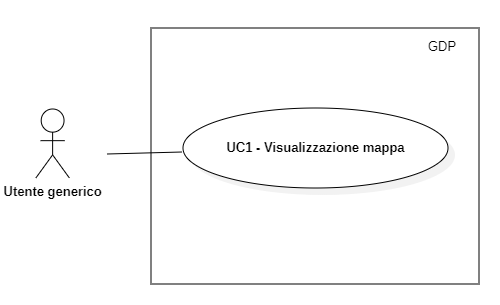
\includegraphics[width=0.95\linewidth]{../immagini/attori_casi/vis_mappa.png}
		\caption{UC1 - Visualizzazione mappa}
	\end{figure}
\end{center}
\begin{itemize}
	\item \textbf{Attori primari}: utente generico;
	\item \textbf{Descrizione}: l'utente visualizza una mappa presente nell'applicazione web. Tale mappa è una heat map e presenta all'utente i dati analizzati dal prodotto;
	\item \textbf{Scenario principale}: l'utente accede all'applicazione web e visualizza la mappa;
	\item \textbf{Precondizione}: il sistema è attivo e funzionante;
	\item \textbf{Postcondizione}: il sistema invia i dati alla pagina al caricamento presentando una mappa con tutti i dati per l'utente.
\end{itemize}
\begin{center}
	\begin{figure}[H]
		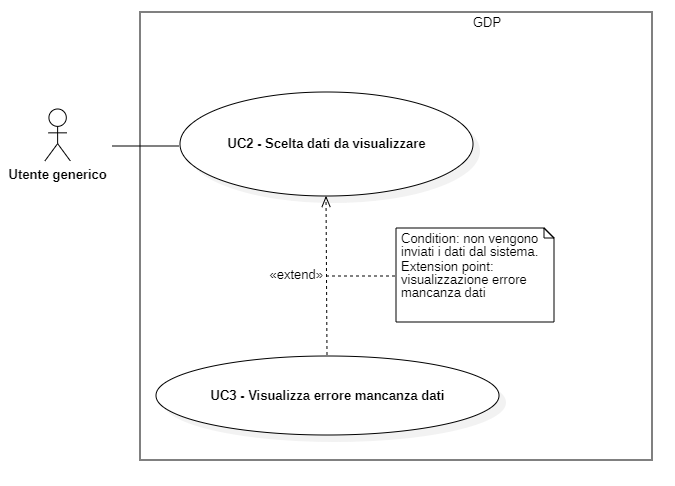
\includegraphics[width=0.95\linewidth]{../immagini/attori_casi/uc2.png}
		\caption{Schema generale: Scelta dati da visualizzare ed errori}
	\end{figure}
\end{center}
\subsection{UC2 - Scelta dati da visualizzare}
\begin{center}
	\begin{figure}[H]
		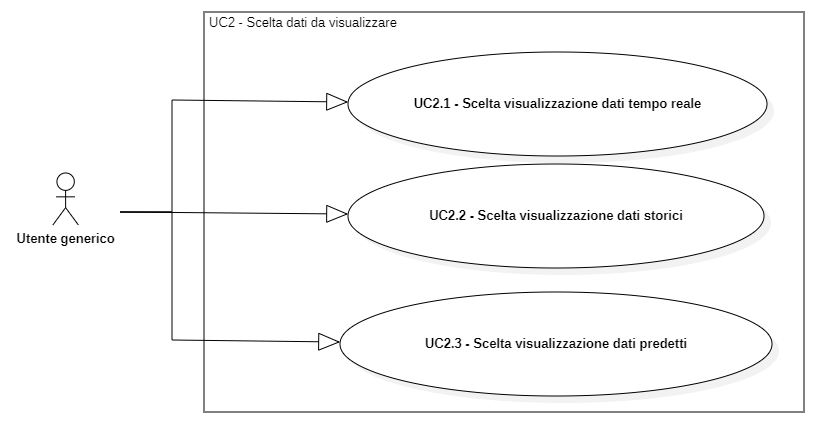
\includegraphics[width=0.95\linewidth]{../immagini/attori_casi/uc2_1_2_3.png}
		\caption{UC2 - Scelta dati da visualizzare}
	\end{figure}
\end{center}

\begin{itemize}
	\item \textbf{Attori primari}: utente generico;
	\item \textbf{Descrizione}: l'utente sceglie la tipologia di dati disponibili da rappresentare nella mappa;
	\item \textbf{Scenario principale}: l'utente accede all'applicazione web e seleziona il tipo di dato da visualizzare. Il sistema fornisce i dati alla mappa e viene così aggiornata;
	\item \textbf{Estensione}: 
	\begin{itemize}
		\item \textbf{UC3}: se l'applicazione web non riceve nessuna informazione dal sistema viene visualizzato un messaggio di errore.
	\end{itemize}
	\item \textbf{Precondizione}: il sistema è attivo e funzionante e l'utente sceglie la tipologia di dati da utilizzare;
	\item \textbf{Postcondizione}: il sistema invia i dati all'applicazione web e aggiorna la mappa in base alle nuove informazioni.
\end{itemize}

\subsection{UC2.1 - Scelta visualizzazione dati in tempo reale}
\begin{itemize}
	\item \textbf{Attori primari}: utente generico;
	\item \textbf{Descrizione}: l'utente sceglie la tipologia dati in tempo reale da rappresentare nella mappa;
	\item \textbf{Scenario principale}: l'utente accede all'applicazione web e seleziona la visualizzazione dati in tempo reale. Il sistema fornisce solo i dati richiesti alla mappa e viene così aggiornata;
	\item \textbf{Precondizione}: il sistema è attivo e funzionante e i dati in tempo reale sono presenti nel sistema;
	\item \textbf{Postcondizione}: il sistema invia i dati in tempo reale all'applicazione web e aggiorna la mappa in base alle nuove informazioni.
\end{itemize}

\subsection{UC2.2 - Scelta visualizzazione dati storici}
\begin{itemize}
	\item \textbf{Attori primari}: utente generico;
	\item \textbf{Descrizione}: l'utente sceglie la tipologia dati storici da rappresentare nella mappa;
	\item \textbf{Scenario principale}: l'utente accede all'applicazione web e seleziona la visualizzazione dati storici. Il sistema fornisce solo i dati richiesti alla mappa e viene così aggiornata;
	\item \textbf{Precondizione}: il sistema è attivo e funzionante e i dati storici sono presenti nel sistema;
	\item \textbf{Postcondizione}: il sistema invia i dati storici all'applicazione web e aggiorna la mappa in base alle nuove informazioni.
\end{itemize}

\subsection{UC2.3 - Scelta visualizzazione dati predetti}
\begin{itemize}
	\item \textbf{Attori primari}: utente generico;
	\item \textbf{Descrizione}: l'utente sceglie la tipologia dati con predizione da rappresentare nella mappa;
	\item \textbf{Scenario principale}: l'utente accede all'applicazione web e seleziona la visualizzazione dati con predizione. Il sistema fornisce solo i dati richiesti alla mappa e viene così aggiornata;
	\item \textbf{Precondizione}: il sistema è attivo e funzionante e i dati elaborati dal modello di \textit{machine learning} sono presenti nel sistema;
	\item \textbf{Postcondizione}: il sistema invia i dati predetti all'applicazione web e aggiorna la mappa in base alle nuove informazioni.
\end{itemize}

\subsection{UC3 - Visualizza errore mancanza dati}
\begin{itemize}
	\item \textbf{Attori primari}: utente generico;
	\item \textbf{Descrizione}: l'utente visualizza un messaggio di errore in quanto vi è una mancanza di dati dal sistema;
	\item \textbf{Scenario principale}: l'utente dopo essere entrato nell'applicazione web, seleziona un tipologia di dati da visualizzare nella mappa e il sistema non riesce a completare la richiesta;
	\item \textbf{Precondizione}: i dati richiesti non sono presenti nel sistema;
	\item \textbf{Postcondizione}: il sistema invia un messaggio di errore per informare l'utente che i dati richiesti non sono disponibili.
\end{itemize}

\chapter{Requisiti}\label{Requisiti}
In questa sezione vengono illustrati attraverso una tabella tutti i requisiti$_{\scaleto{G}{3pt}}$ individuati dal proponente$_{\scaleto{G}{3pt}}$ e dal gruppo \textit{Jawa Druids}. Ogni requisito viene individuato da un codice identificativo, una sua descrizione, la tipologia di requisito e la fonte di riferimento, la spiegazione di ogni parte è descritta nel documento \textit{Norme del Progetto v1.0.0}. Nella sezione successiva viene illustrato attraverso una tabella il tracciamento dei requisiti alla loro fonte e viceversa.

\section{Requisiti funzionali}\label{RequisitiFunzionali}

\def\tabularxcolumn#1{m{#1}}
{\rowcolors{2}{RawSienna!90!RawSienna!20}{RawSienna!70!RawSienna!40}

	\begin{center}
		\renewcommand{\arraystretch}{1.4}
		\begin{longtable}{|p{3cm}|p{4cm}|p{4cm}|p{4cm}|}
			\hline
			\rowcolor{airforceblue}
			\makecell[c]{\textbf{Codice RS}} & \makecell[c]{\textbf{Descrizione}} & \makecell[c]{\textbf{Tipo di requisito}} & \makecell[c]{\textbf{Fonte}} \\
			%fase 1
			\hline
			\centering RSFO1 & Realizzazione di motori software ‘contapersone’  &\centering  Obbligatorio & \makecell[tc]{Capitolato$_{\scaleto{G}{3pt}}$ \\ V. esterno 17-12-2020 } \\
			% \shortstack{Capitolato\\Verbale esterno 17-12-2020}   \\
			\hline
			\centering RSFF2 & Realizzazione di simulatori di altre sorgenti dati sia dei dati storici/in monitoraggio che dati previsionali & \centering Facoltativo & \makecell[tc]{Capitolato$_{\scaleto{G}{3pt}}$ } \\
			\hline
			\centering RSFO3  & Viene visualizzato un messaggio di errore per la mancanza dati nella generazione della heat-map  &\centering  Obbligatorio & \makecell[tc]{UC2}  \\
			\hline
			\centering RSFO4 & Archiviazione di tutti i dati nel database & \centering Obbligatorio & \makecell[tc]{Capitolato$_{\scaleto{G}{3pt}}$ \\ UC5}  \\
			\hline
			\centering RSFO4.1 & Archiviazione di tutti i dati reali nel database & \centering Obbligatorio & \makecell[tc]{Capitolato$_{\scaleto{G}{3pt}}$ \\ UC5.1 \\ UC5.2}  \\
			\hline
			\centering RSFO4.2 & Archiviazione di tutti i dati elaborati dal modello ML nel database & \centering Obbligatorio & \makecell[tc]{Capitolato$_{\scaleto{G}{3pt}}$ \\ UC5.3}  \\
			%fase 2
			\hline
			\centering RSFO5 & Elaborazione in tempo reale dei dati acquisiti da flussi esterni &\centering  Obbligatorio & \makecell[tc]{Capitolato$_{\scaleto{G}{3pt}}$}  \\
			\hline
			\centering RSFD5.1 & Identificazione di eventi che portano alla variazione del flusso di utenti &\centering  Desiderabile & \makecell[tc]{Capitolato$_{\scaleto{G}{3pt}}$}  \\
			\hline
			\centering RSFD6 & Previsione dell'insorgenza futura di variazioni significative di flussi di persone & \centering Desiderabile & \makecell[tc]{Capitolato$_{\scaleto{G}{3pt}}$ }  \\
			%fase 3
			\hline
			\centering RSFO7 & Visualizzazione dei dati elaborati attraverso heat map$_{\scaleto{G}{3pt}}$ &\centering  Obbligatorio & \makecell[tc]{Capitolato$_{\scaleto{G}{3pt}}$ \\ UC1}  \\
			\hline
			\centering RSFO8 & Apache Kafka$_{\scaleto{G}{3pt}}$ deve creare una comunicazione tra il programma con il software 'contapersone' e il database  &\centering  Obbligatorio &  \makecell[tc]{Interno} 	\\
			\hline
			\centering RSFO9 & L'utente deve poter visualizzare i dati in tempo reale tramite heat map$_{\scaleto{G}{3pt}}$  &\centering  Obbligatorio &  \makecell[tc]{Interno \\ UC1} 	\\
			\hline
			\centering RSFO10 & L'utente deve poter visualizzare i dati storicizzati tramite heat map$_{\scaleto{G}{3pt}}$  &\centering  Obbligatorio &  \makecell[tc]{Interno \\ UC1} 	\\
			\hline
			\centering RSFO11 & L'utente deve poter visualizzare una previsione tramite heat map$_{\scaleto{G}{3pt}}$  &\centering  Obbligatorio &  \makecell[tc]{Interno \\ UC1} 	\\
			\hline
			\centering RSFF12 & L'utente deve poter distinguere fra i dati simulati e quelli reali  &\centering  Facoltativo &  \makecell[tc]{Interno} 	\\
			\hline
			\centering RSFD13 & L'utente deve poter visualizzare un indice di affidabilità della previsione nella mappa  &\centering  Desiderabile &  \makecell[tc]{Interno} 	\\ 
			\hline
			\centering RSFD14 & L'utente deve poter visualizzare un indice di affidabilità dei dati in tempo reale nella mappa  &\centering  Desiderabile &  \makecell[tc]{Interno} 	\\
			\hline
			\centering RSFF15 & L'utente deve poter applicare dei filtri ai dati (reali, simulati)  &\centering  Facoltativo &  \makecell[tc]{Interno } 	\\
			\hline
			\centering RSFF16 & L'utente ha la possibilità di scegliere le sorgenti dati da cui prelevare dati  &\centering  Facoltativo &  \makecell[tc]{Interno} 	\\
			\hline
			\centering RSFO17 & Il sistema deve aggiornare la mappa automaticamente ogni 10 minuti &\centering Obbligatorio & \makecell[tc]{Interno} \\
			\hline
			\centering RSFO18 & Il modello di machine learning$_{\scaleto{G}{3pt}}$ deve poter salvare i pesi e le predizioni in un file & \centering Obbligatorio &  \makecell[tc]{V. esterno 2-02-2021} \\
			\hline
			\centering RSFO18.1 & Il formato di file prodotto deve essere .h5 & \centering Obbligatorio & \makecell[tc]{V. esterno 2-02-2021} \\
			\hline
			\centering RSFO19 & Viene inviato un messaggio di errore al front end, dal back end, se non ci sono i dati richiesti &\centering Obbligatorio & \makecell[tc]{Interno \\ UC6} \\
			\hline
			\centering RSFO20 & L'utente può selezionare una città tra quelle disponibili &\centering Obbligatorio & \makecell[tc]{Interno \\ UC3} \\
			\hline
			\centering RSFO21 & Le zone visualizzate della città dipendono dalle sorgenti esterne utilizzate &\centering Obbligatorio & \makecell[tc]{Interno} \\
			\hline
			\centering RSFO22  & I dati acquisiti da telecamere in tempo reale devono avere data di riferimento associata  &\centering Obbligatorio & \makecell[tc]{Interno} \\
			\hline
			\centering RSFO22.1  & I dati acquisiti da telecamere in tempo reale devono avere un orario di riferimento associato &\centering Obbligatorio & \makecell[tc]{Interno} \\
			\hline
			\centering RSFO22.2  & I dati acquisiti da telecamere in tempo reale devono avere un luogo di riferimento associato &\centering Obbligatorio  & \makecell[tc]{Interno} \\
			\hline
			\centering RSFF23 & Possibilità da parte del sistema di scegliere di mostrare i dati predetti in caso di mancanza di quelli reali &\centering Facoltativo & \makecell[tc]{Interno} \\
			\hline
			\centering RSFO24 & La selezione dell'orario è effettuata su intervalli di tempo di ora in ora &\centering Obbligatorio & \makecell[tc]{UC4.1} \\
			\hline
			\centering RSFO25 & Il sistema dà priorità ai dati reali presenti nel database per la visualizzazione della mappa su periodi di tempo storici &\centering Obbligatorio & \makecell[tc]{Interno} \\
			\hline
			\centering RSFO26 & Il sistema aggiorna automaticamente la mappa alla selezione di un diverso orario &\centering Obbligatorio & \makecell[tc]{UC4.1} \\
			\hline
			\centering RSFO27 & L'utente deve poter selezionare la data del giorno di cui vuole visualizzare i dati   &\centering Obbligatorio & \makecell[tc]{UC4.2} \\
			\hline
			\centering RSFO28 & L'utente deve poter ripristinare la visione in tempo reale tramite un pulsante di ripristino &\centering Obbligatorio & \makecell[tc]{UC4.3} \\
			\hline
			\centering RSFD29 & Il sistema deve poter prelevare dati da diverse fonti e formattarle nel tipo di default &\centering Desiderabile & \makecell[tc]{Interno} \\
			\hline
			\centering RSFO30 & Il sistema deve utilizzare un software 'contapersone' già allenato &\centering Obbligatorio & \makecell[tc]{V. esterno 28-01-2021} \\
			\hline
			\rowcolor{white}
			\caption[Requisiti funzionali]{Requisiti funzionali}\label{4.1}\\
	\end{longtable}%\captionof{table}{Requisiti funzionali}

\end{center}

\section{Requisiti prestazionali}\label{RequisitiPrestazionali}
\def\tabularxcolumn#1{m{#1}}
{\rowcolors{2}{RawSienna!90!RawSienna!20}{RawSienna!70!RawSienna!40}

	\begin{center}
		\renewcommand{\arraystretch}{1.4}
		\begin{longtable}{|p{4cm}|p{4cm}|p{4cm}|p{3cm}|}
		\hline
		\rowcolor{airforceblue}
		\makecell[c]{\textbf{Codice RS}} & \makecell[c]{\textbf{Descrizione}} & \makecell[c]{\textbf{Tipo di requisito}} & \makecell[c]{\textbf{Fonte}} \\
		\hline
		\centering RSPO1 & Capacità di acquisizione continuativa nel tempo dei dati da flussi esterni, viene prelevato almeno un dato ogni 10 minuti &\centering  Obbligatorio & \makecell[tc]{Capitolato$_{\scaleto{G}{3pt}}$}  \\
		\hline
		\centering RSPO2 & Modalità a bassa latenza nell'aquisizione di informazioni, almeno un dato ogni 5 minuti assumendo una connessione con download di minimo 100kb/s & \centering Obbligatorio & \makecell[tc]{Interno} \\
		\hline
		\centering RSPO3 & Modalità a bassa latenza per l'elaborazione dei dati acquisiti, almeno una elaborazione ogni 4 minuti & \centering Obbligatorio & \makecell[tc]{Interno} \\
		\hline
		\centering RSPO4 & Modalità a bassa latenza per la visualizzazione delle informazioni, la mappa si aggiorna in massimo 30s & \centering Obbligatorio & \makecell[tc]{Interno} \\
		\hline
		\centering RSPF5 & Misurazione indice di affidabilità sui dati in tempo reale di almeno 75\% & \centering Facoltativo &\makecell[tc]{Interno} \\
		\hline
		\rowcolor{white}
		
		\caption[Requisiti prestazionali]{Requisiti prestazionali}\label{4.2}\\
			\end{longtable}
	\end{center}
\section{Requisiti di qualità}\label{RequisitiDiQualita}
\def\tabularxcolumn#1{m{#1}}
{\rowcolors{2}{RawSienna!90!RawSienna!20}{RawSienna!70!RawSienna!40}

	\begin{center}
		\renewcommand{\arraystretch}{1.4}
		\begin{longtable}{|p{4cm}|p{4cm}|p{4cm}|p{3cm}|}
			\hline
			\rowcolor{airforceblue}
			\makecell[c]{\textbf{Codice RS}} & \makecell[c]{\textbf{Descrizione}} & \makecell[c]{\textbf{Tipo di requisito}} & \makecell[c]{\textbf{Fonte}} \\
			\hline
		\centering RSQO1  & La progettazione e la codifica dei requisiti devono rispettare le norme e le metriche definite nel documento \textit{Norme di Progetto v1.0.0}&\centering  Obbligatorio & \makecell[tc]{Interno} \\
		\hline
		\centering RSQF2  & Il codice sorgente del software deve essere disponibile in una repository$_G$ pubblica su Github$_G$  &\centering  Facoltativo & \makecell[tc]{Interno} \\
		\hline
		\centering RSQF3  & Deve essere sviluppato e fornito un documento con lo schema della base di dati relazionale  & \centering Facoltativo & \makecell[tc]{Interno } \\
	%	\hline
	%	RSQ  & Fornire una documentazione sui flussi di dati esterni.... & Facoltativo & FC3 \\
	%	\hline
		\hline
		\centering RSQF4  & Deve essere realizzato un documento contenente tutti gli errori risolti durante la realizzazione del software &\centering  Facoltativo & \makecell[tc]{Interno} \\
		\hline
		\centering RSQO5  & Test che dimostrino il corretto funzionamento dei servizi e delle funzionalità previste  & \centering Obbligatorio & \makecell[tc]{Capitolato$_{\scaleto{G}{3pt}}$} \\
		\hline
		\centering RSQO6  & Dev'essere disponibile un manuale sviluppatore  & \centering Obbligatorio & \makecell[tc]{Capitolato$_{\scaleto{G}{3pt}}$} \\
		\hline
		\centering RSQO7  & Dev'essere disponibile un manuale utente  & \centering Obbligatorio & \makecell[tc]{Capitolato$_{\scaleto{G}{3pt}}$} \\
		\hline
		\rowcolor{white}

		\caption[Requisiti di qualità]{Requisiti di qualità}\label{4.3}\\
		\end{longtable}
\end{center}

\newpage
\section{Requisiti di vincolo}\label{RequisitiVincolo}
\def\tabularxcolumn#1{m{#1}}
{\rowcolors{2}{RawSienna!90!RawSienna!20}{RawSienna!70!RawSienna!40}

\begin{center}
	\renewcommand{\arraystretch}{1.4}
	\begin{longtable}{|p{3cm}|p{4cm}|p{4cm}|p{4cm}|}
		\hline
		\rowcolor{airforceblue}
		\makecell[c]{\textbf{Codice RS}} & \makecell[c]{\textbf{Descrizione}} & \makecell[c]{\textbf{Tipo di requisito}} & \makecell[c]{\textbf{Fonte}} \\
		\hline
		\centering RSVO1  & Il front-end$_{\scaleto{G}{3pt}}$ del prodotto viene sviluppato utilizzando tecnologie web &\centering Obbligatorio  & \makecell[tc]{Capitolato$_{\scaleto{G}{3pt}}$} \\
		\hline
		\centering RSVF1.1  & Utilizzo di leaflet.js$_{\scaleto{G}{3pt}}$ per la creazione di heat map$_{\scaleto{G}{3pt}}$ &\centering  Facoltativo & \makecell[tc]{Capitolato$_{\scaleto{G}{3pt}}$} \\
		\hline
		\centering RSVO1.2  & Utilizzo di vue.js$_{\scaleto{G}{3pt}}$ per la creazione della wep-app$_{\scaleto{G}{3pt}}$  &\centering  Obbligatorio  & \makecell[tc]{V. esterno 02-01-2021} \\
		\hline
		\centering RSVO3  & Il sistema deve far uso dell'ecosistema Apache Kafka$_{\scaleto{G}{3pt}}$ &\centering  Obbligatorio  & \makecell[tc]{Capitolato$_{\scaleto{G}{3pt}}$} \\
		\hline
		\centering RSVO4  & Il back end$_{\scaleto{G}{3pt}}$ del prodotto viene sviluppato utilizzando il linguaggio Java$_{\scaleto{G}{3pt}}$ &\centering  Obbligatorio  & \makecell[tc]{Capitolato$_{\scaleto{G}{3pt}}$} \\
		\hline
		\centering RSVO5  & Supporto browser Chrome, Firefox con versioni massimo di 3 anni &\centering  Obbligatorio  & \makecell[tc]{Interno} \\
		\hline
		\centering RSVF6  & Supporto browser Safari, Microsoft Edge &\centering  Facoltativo  & \makecell[tc]{Interno} \\
		\hline
		\centering RSVO7  & La web application dev'essere disponibile in un ambiente locale, di sviluppo, e di produzione & \centering  Obbligatorio  & \makecell[tc]{Capitolato$_{\scaleto{G}{3pt}}$} \\
		\hline
		\centering RSVF8 & Utilizzo di Keras per lo sviluppo del modello machine learning$_{\scaleto{G}{3pt}}$ & \centering Facoltativo & \makecell[tc]{V. esterno 02-02-2021} \\
		\hline
		\centering RSVF9 & Utilizzo di Pandas come strumento per la manipolazione dei dati & \centering Facoltativo & \makecell[tc]{V. esterno 02-02-2021} \\
		\hline
		\rowcolor{white}

		\caption[Requisiti di vincolo]{Requisiti di vincolo}\label{4.4}\\
	\end{longtable}
\end{center}

\section{Tracciamento dei requisiti}\label{RequisitiTracciamentoDeiRequisiti}

\subsection{Requisito - fonte}\label{RequisitiTracciamentoDeiRequisitiFonte}

\def\tabularxcolumn#1{m{#1}}
{\rowcolors{2}{RawSienna!90!RawSienna!20}{RawSienna!70!RawSienna!40}
	\begin{center}
		\renewcommand{\arraystretch}{1.4}
		\begin{longtable}{|p{7.5cm}|p{7.5cm}|}
		\hline
		\rowcolor{airforceblue}
		\makecell[tc]{\textbf{Codice RS}} & \makecell[c]{\textbf{Fonte}}  \\
		\hline
		\makecell[tc]{RSFO1} & \makecell[tc]{Capitolato$_{\scaleto{G}{3pt}}$\\V. esterno 17-12-2020} \\
		\hline
		\makecell[tc]{RSFF2} & \makecell[tc]{Capitolato$_{\scaleto{G}{3pt}}$}\\
		\hline
		\makecell[tc]{RSFO3.1} & \makecell[tc]{Interno \\ UC3}\\
		\hline
		\makecell[tc]{RSFO4.1} & \makecell[tc]{Capitolato$_{\scaleto{G}{3pt}}$\\UC2}\\
		\hline
		\makecell[tc]{RSFO4.2} & \makecell[tc]{Capitolato$_{\scaleto{G}{3pt}}$\\UC2}\\
		\hline
		\makecell[tc]{RSFO5} & \makecell[tc]{Capitolato$_{\scaleto{G}{3pt}}$}\\
		\hline
		\makecell[tc]{RSFO5.1} & \makecell[tc]{Capitolato$_{\scaleto{G}{3pt}}$}\\ 
		\hline
		\makecell[tc]{RSFD6}& \makecell[tc]{Capitolato$_{\scaleto{G}{3pt}}$}\\
		\hline
		\makecell[tc]{RSFO7} & \makecell[tc]{Capitolato$_{\scaleto{G}{3pt}}$\\UC1}\\
		\hline
		\makecell[tc]{RSFO8} & \makecell[tc]{Interno}\\ 
		\hline
		\makecell[tc]{RSFO9} & \makecell[tc]{Interno \\ UC5}\\
		\hline
		\makecell[tc]{RSFO10} & \makecell[tc]{Interno \\ UC5}\\
		\hline
		\makecell[tc]{RSFO11} & \makecell[tc]{Interno \\ UC5}\\
		\hline
		\makecell[tc]{RSFF12} & \makecell[tc]{Interno \\ UC1}\\
		\hline
		\makecell[tc]{RSFD13} & \makecell[tc]{Interno}\\
		\hline
		\makecell[tc]{RSFD14} & \makecell[tc]{Interno}\\
		\hline
		\makecell[tc]{RSFF15} & \makecell[tc]{Interno}\\
		\hline
		\makecell[tc]{RSFF16} & \makecell[tc]{Interno}\\
		\hline
		\makecell[tc]{RSFO17} & \makecell[tc]{Interno \\ UC1}\\
		\hline
		\makecell[tc]{RSFO18} & \makecell[tc]{Interno \\ UC3.2}\\
		\hline
		\makecell[tc]{RSFO19} & \makecell[tc]{Interno \\ UC3.3}\\
		\hline
		\makecell[tc]{RSFO20} & \makecell[tc]{Interno \\ UC4}\\
		\hline
		\makecell[tc]{RSFO21} & \makecell[tc]{Interno}\\
		\hline
		\makecell[tc]{RSFO22} & \makecell[tc]{Interno}\\
		\hline
		\makecell[tc]{RSFO22.1} & \makecell[tc]{Interno}\\
		\hline
		\makecell[tc]{RSFO22.2} & \makecell[tc]{Interno}\\
		\hline
		\makecell[tc]{RSFF23} & \makecell[tc]{Interno}\\
		\hline
		\makecell[tc]{RSFO24} & \makecell[tc]{UC5.1}\\
		\hline
		\makecell[tc]{RSFO25} & \makecell[tc]{Interno}\\
		\hline
		\makecell[tc]{RSFO26} & \makecell[tc]{UC5.1}\\
		\hline
		\makecell[tc]{RSFO27} & \makecell[tc]{UC5.2}\\
		\hline
		\makecell[tc]{RSFO28} & \makecell[tc]{UC5.3}\\
		\hline
		\makecell[tc]{RSFD29} & \makecell[tc]{Interno}\\
		\hline
		\makecell[tc]{RSFO30} & \makecell[tc]{V. esterno 28-01-2021}\\
		\hline
		\makecell[tc]{RSFO31} & \makecell[tc]{V. esterno 02-02-2021}\\
		\hline
		\makecell[tc]{RSFO31.1} & \makecell[tc]{V. esterno 02-02-2021}\\ % <-da qui aiuto
		\hline
		\makecell[tc]{RSPO1} & \makecell[tc]{Capitolato$_{\scaleto{G}{3pt}}$}\\
		\hline
		\makecell[tc]{RSPO2} & \makecell[tc]{Capitolato$_{\scaleto{G}{3pt}}$}\\
		\hline
		\makecell[tc]{RSPO3} & \makecell[tc]{}\\
		\hline
		\makecell[tc]{RSPO4} & \makecell[tc]{}\\
		\hline
		\makecell[tc]{RSPO5} & \makecell[tc]{}\\%<- aiuto fine
		\hline
		\makecell[tc]{RSQO1} & \makecell[tc]{Interno}\\
		\hline
		\makecell[tc]{RSQF2} & \makecell[tc]{Interno}\\
		\hline
		\makecell[tc]{RSQF3} & \makecell[tc]{Interno }\\
		\hline
		\makecell[tc]{RSQF4} & \makecell[tc]{Interno}\\
		\hline
		\makecell[tc]{RSQO5} & \makecell[tc]{Capitolato$_{\scaleto{G}{3pt}}$}\\
		\hline
		\makecell[tc]{RSQO6} & \makecell[tc]{Capitolato$_{\scaleto{G}{3pt}}$}\\
		\hline
		\makecell[tc]{RSQO7} & \makecell[tc]{Capitolato$_{\scaleto{G}{3pt}}$}\\
		\hline
		\makecell[tc]{RSVO1} & \makecell[tc]{Interno}\\
		\hline
		\makecell[tc]{RSVO1.1} & \makecell[tc]{Interno}\\
		\hline
		\makecell[tc]{RSVO1.2} & \makecell[tc]{Interno}\\
		\hline
		\makecell[tc]{RSVO2} & \makecell[tc]{Capitolato$_{\scaleto{G}{3pt}}$}\\
		\hline
		\makecell[tc]{RSVF2.1} & \makecell[tc]{Capitolato$_{\scaleto{G}{3pt}}$}\\
		\hline
		\makecell[tc]{RSVO2.2} & \makecell[tc]{Capitolato$_{\scaleto{G}{3pt}}$}\\
		\hline
		\makecell[tc]{RSVO3} & \makecell[tc]{Capitolato$_{\scaleto{G}{3pt}}$}\\
		\hline
		\makecell[tc]{RSVO4} & \makecell[tc]{Capitolato$_{\scaleto{G}{3pt}}$}\\
		\hline
		\makecell[tc]{RSVO5} & \makecell[tc]{Interno}\\
		\hline
		\makecell[tc]{RSVF6} & \makecell[tc]{Interno}\\
		\hline
		\makecell[tc]{RSVO7} & \makecell[tc]{Capitolato$_{\scaleto{G}{3pt}}$}\\
		\hline
		\makecell[tc]{RSVF8} & \makecell[tc]{V. esterno 02-02-2021}\\
		\hline
		\makecell[tc]{RSVF9} & \makecell[tc]{V. esterno 02-02-2021}\\
		\hline
		\rowcolor{white}

		\caption[Tabella tracciamento requisito-fonte]{Tabella tracciamento requisito-fonte}\label{4.5}\\
	\end{longtable}
\end{center}
\clearpage
\subsection{Fonte - requisito}\label{RequisitiTracciamentoDeiRequisitiFonteRequisito}
\def\tabularxcolumn#1{m{#1}}
{\rowcolors{2}{RawSienna!90!RawSienna!20}{RawSienna!70!RawSienna!40}
	\begin{center}
		\renewcommand{\arraystretch}{1.4}
		\begin{longtable}{|p{7.5cm}|p{7.5cm}|}
		\hline
		\rowcolor{airforceblue}
		\makecell[c]{\textbf{Fonte}} & \makecell[c]{\textbf{Codice RS}}  \\
		\hline
		\makecell[c]{Capitolato$_{\scaleto{G}{3pt}}$} & \makecell[c]{RSFO1\\RSFF2\\RSFO4.1\\RSFO4.2\\RSFO5\\RSFO5.1\\RSFD6\\RSFO7\\RSPO1\\RSPO2\\RSQO5\\RSQO6\\RSQO7\\RSVO2\\RSVF2.1\\RSVO2.2\\RSVO3\\RSVO4\\RSVO7} \\
		\hline
		\makecell[c]{UC1} & \makecell[c]{RSFO7 \\ RSFF12 \\ RSFO17} \\
		\hline
		\makecell[c]{UC2} & \makecell[c]{RSFO4.1 \\ RSFO4.2 } \\
		\hline
		\makecell[c]{UC3} & \makecell[c]{RSVO3.1 } \\ % UC3.2 RSFO18, UC3.3 RSFO19
		\hline
		\makecell[c]{UC4} & \makecell[c]{RSFO20 } \\
		\hline
		\makecell[c]{UC5} & \makecell[c]{RSFO9 \\ RSFO10 \\ RSFO11} \\
		\hline
		\makecell[c]{UC5.1} & \makecell[c]{RSFO24 \\ RSFO26 } \\
		\hline
		\makecell[c]{UC5.2} & \makecell[c]{RSFO27  } \\
		\hline
		\makecell[c]{UC5.3} & \makecell[c]{RSFO28 } \\
		\hline
		\makecell[c]{Interno} &\makecell[c]{RSFO3.1\\RSFO8\\RSFO9\\RSFO10\\RSFO11\\RSFF12\\RSFD13\\RSFD14\\RSFF15\\RSFF16\\RSFO17\\RSFO18\\RSFO19\\RSFO20\\RSFO8\\RSQO1\\RSQF2\\RSQF3\\RSQF4\\RSVO1\\RSVO1.1\\RSVO1.2} \\
		\hline
		\makecell[c]{Verbale esterno 17-12-2020} & \makecell[c]{RSFO1} \\
		\hline
		\rowcolor{white}

		\caption[Tabella tracciamento fonte-requisito]{Tabella tracciamento fonte-requisito}\label{4.6}\\
	\end{longtable}
\end{center}

\section{Considerazioni}\label{requisitiConsiderazioni}
I requisiti potranno subire delle variazioni in futuro, in modo tale da apportare degli aggiornamenti alle voci presenti o delle migliorie.
Nel caso in cui le attività pianificate terminassero prima del previsto e dovessero avanzare delle ore di lavoro, potranno essere presi in carico nuovi requisiti per aggiungere del valore al prodotto. Pertanto, qualsiasi espansione è riservata solo per il futuro.

%PER RENDERE PIÙ CHIARA LA STESURA DEI DOCUMENTI È MEGLIO LASCIARE SEPARATI IN FILE DIVERSI OGNI CAPITOLO

% \input{esempio} -- esempio di codice per inserire un nuovo capitolo

\end{document}